
%(BEGIN_QUESTION)
% Copyright 2015, Tony R. Kuphaldt, released under the Creative Commons Attribution License (v 1.0)
% This means you may do almost anything with this work of mine, so long as you give me proper credit

Explain how to isolate the protective relay from all PTs and all CTs prior to testing the relay:

$$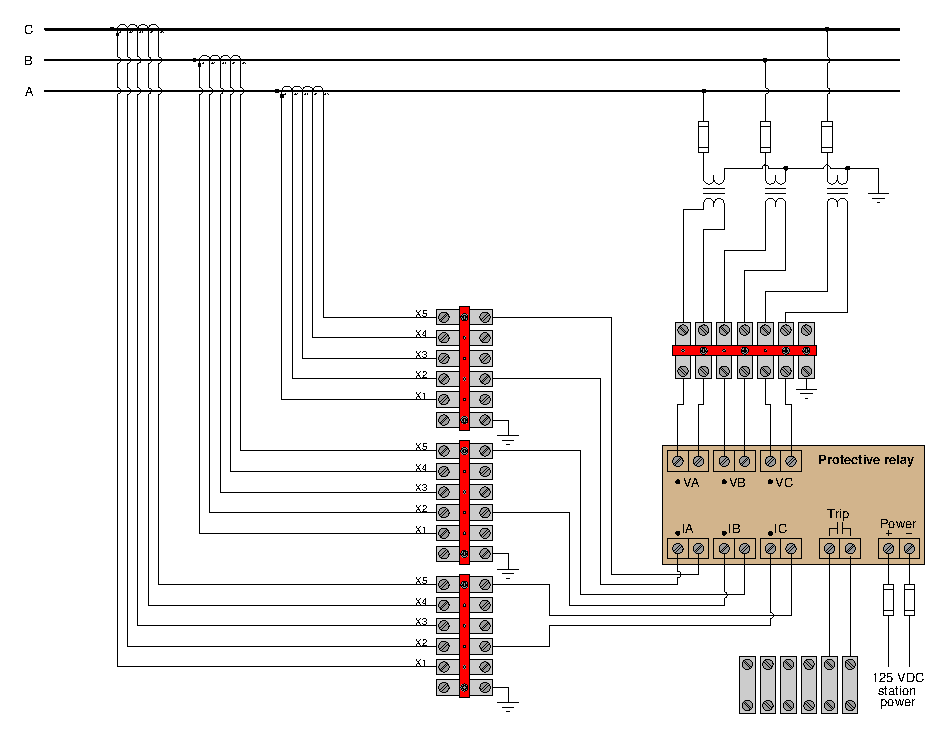
\includegraphics[width=15.5cm]{i02883x01.eps}$$


\underbar{file i02883}
%(END_QUESTION)





%(BEGIN_ANSWER)

 
%(END_ANSWER)





%(BEGIN_NOTES)

We must add shorting screws to the CT terminal blocks (at the X2 position), then we may disconnect the ungrounded wire between those terminal blocks and the relay.  No shorting screws are necessary for the PT circuits, and in fact would destroy the PTs if added!

$$\includegraphics[width=15.5cm]{i02883x02.eps}$$

%INDEX% Protective relay: shorting terminal block

%(END_NOTES)


